\documentclass[aps,pra,notitlepage,amsmath,amssymb,letterpaper,12pt]{revtex4-1}
\usepackage{amsthm}
\usepackage{graphicx}
%  Above uses the Americal Physical Society template for Physical Review A
%  as a reasonable and fully-featured default template
 
%  Below define helpful commands to set up problem environments easily
\newenvironment{problem}[2][Problem]{\begin{trivlist}
\item[\hskip \labelsep {\bfseries #1}\hskip \labelsep {\bfseries #2.}]}{\end{trivlist}}
\newenvironment{solution}{\begin{proof}[Solution]}{\end{proof}}
 
% --------------------------------------------------------------
%                   Document Begins Here
% --------------------------------------------------------------
 
\begin{document}
 
\title{Introduction to Derivatives}
\author{Aly and Seong}
\affiliation{CS 510, Schmid College of Science and Technology, Chapman University}
\date{\today}

\maketitle

\section{Derivative Basics} % Specify main sections this way

% x.yz is the problem number
\begin{problem}{x.yz} 
What is the definition of a derivative?
\end{problem}
 
\begin{solution} %You can also use proof in place of solution
The derivative, f'(x), for a function, f(x), is
\begin{align}
\frac{d}{{dx}}f\left( x \right) = \mathop {\lim }\limits_{\Delta \to 0} \frac{{f\left( {x + \Delta } \right) - f\left( x \right)}}{\Delta }
\end{align}
% Use align environments for equations. The \\ is a newline character. The & is the alignment character.
% Using align* or \nonumber on each line removes equation numbers
\end{solution}

\subsection{Function Diagram} % Specify subsections and subsubsections this way

Diagrams can help in visualizing derivatives. 

\begin{figure}[h!] % h forces the figure to be placed here, in the text
  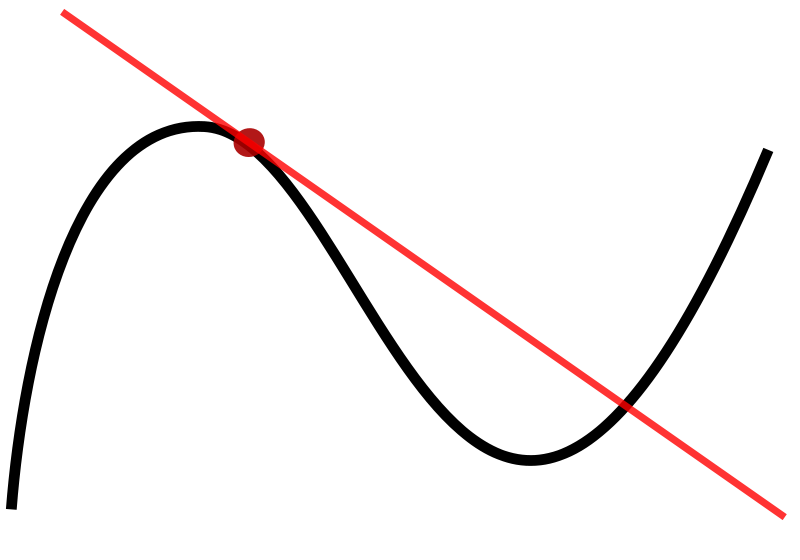
\includegraphics[width=0.4\textwidth]{derivative.png}  % if pdflatex is used, jpg, pdf, and png are permitted
  \caption{The function f(x) is the curve in black with the line tangent to the function drawn in red. The derivative of the function f(x) is the slope of the tangent line shown.}
  \label{fig:figlabel}
\end{figure}

Citations:
https://goo.gl/images/3WSR3k

% Repeat as needed
 
\end{document}

%configuration={"latex_command":"latexmk -pdf -f -g -bibtex -synctex=1 -interaction=nonstopmode 'testlatex.tex'"}
